\documentclass[tikz,dvipsnames]{standalone}
\usetikzlibrary{intersections}

\usepackage{amssymb}
\usepackage{bm}

\begin{document}

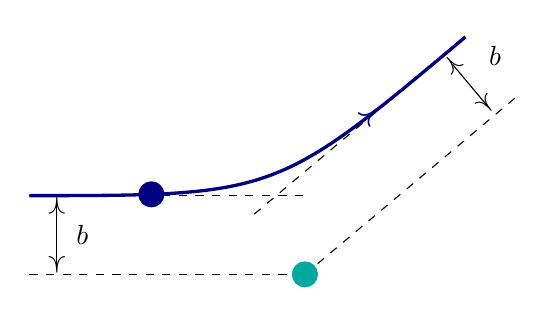
\begin{tikzpicture}
    \draw[dashed, rotate=40] (0,0)--(3.5,0) node[pos=0.9] (e){};
    \draw[dashed, rotate=40, name path=ab] (0,1)--(3.5,1) node[pos=0.9] (d){} node[pos=1] (a){};
    \draw[dashed] (-3.5,0)--(0,0) node[circle,fill=Emerald, pos=1] {} node[pos=0.1] (b){};
    \draw[dashed,name path=cd] (-3.5,1)--(0,1) node[pos=0.1] (c){};
    \draw[very thick, NavyBlue, name intersections={of=ab and cd}]  (-3.5,1)..controls (intersection-1).. (a.center) node[circle,fill=NavyBlue, pos=0.2] {} node[color=NavyBlue, pos=0.8,rotate=40] {$\bm{\succ}$};
    \draw (b)--(c) node[pos=1] {$\curlywedge$} node[pos=0] {$\curlyvee$} node[pos=0.5, label=right:$b$] {};
    \draw (e)--(d) node[pos=1,rotate=40] {$\curlywedge$} node[pos=0, rotate=40] {$\curlyvee$} node[pos=0.5, label=above right:$b$] {};
\end{tikzpicture}

\end{document}